\documentclass[9pt]{beamer}
\usetheme{AnnArbor} %Darmstadt %Warsaw %AnnArbor 
\usecolortheme{spruce} %seahorse 
\usepackage[spanish,mexico]{babel}
\usepackage[utf8]{inputenc}
\usepackage{graphicx}
\usepackage{times}
\usefonttheme{structurebold}
\setbeamercovered{transparent} %transparent %dynamic
\usepackage{subfigure}
\usepackage{amssymb, amsmath, amsbsy}
\usepackage[sort&compress,numbers]{natbib}
\selectlanguage{spanish}
\usepackage[spanish,onelanguage]{algorithm2e}
\usepackage{listings}
\newcounter{saveenumi}
\newcommand{\seti}{\setcounter{saveenumi}{\value{enumi}}}
\newcommand{\conti}{\setcounter{enumi}{\value{saveenumi}}}
\usepackage{tabu}
\extrarowsep = 1mm
\usepackage{multirow}
\usepackage[export]{adjustbox}

\defbeamertemplate*{title page}{propio}[1][]
{
  \vbox{}
  \vfill
  \begingroup
    \centering    
    {\usebeamercolor[fg]{titlegraphic}\inserttitlegraphic\par}
    \vspace{0.1 \paperheight}%
    \begin{beamercolorbox}[sep=8pt,center,#1]{title}
      \usebeamerfont{title}\inserttitle\par%
      \ifx\insertsubtitle\@empty%
      \else%
        \vskip0.25em%
        {\usebeamerfont{subtitle}\usebeamercolor[fg]{subtitle}\insertsubtitle\par}%
      \fi%     
    \end{beamercolorbox}%
    \vskip1em\par
    \begin{beamercolorbox}[sep=8pt,center,#1]{author}
      \usebeamerfont{author}\insertauthor
    \end{beamercolorbox}
    \begin{beamercolorbox}[sep=8pt,center,#1]{institute}
      \usebeamerfont{institute}\insertinstitute
    \end{beamercolorbox}
    \begin{beamercolorbox}[sep=8pt,center,#1]{date}
      \usebeamerfont{date}\insertdate
    \end{beamercolorbox}\vskip0.5em

  \endgroup
  \vfill
}

%https://ondahostil.wordpress.com/2016/11/15/lo-que-he-aprendido-esquemas-en-latex/
\usepackage{schemata}
\newcommand\diagram[2]{\schema{\schemabox{#1}}{\schemabox{#2}}}
\setbeamertemplate{navigation symbols}{}

\graphicspath{ {Figuras/} }  % Las figuras se colocan en la carpeta Figuras
%Recuerde que para agregar la carpeta de figuras se debe ejecutar las fuciones siguientes: pdflatex bibtex pdflatex pdflatex (F6+F11+F6+F6) desde línea de comandos o desde la interfaz que usted utilice. 

\title{Aquí va el Título de la Presentación}
\author{{\bf Nombre Apellido}}
%\institute{\sc Posgrado en Ingeniería con especialidad en Ingeniería de %Sistemas \\
%Facultad de Ingeniería Mecánica y Eléctrica\\
%Universidad Autónoma de Nuevo León}
%\date{\today}

\titlegraphic{
	%\includegraphics[scale=1.0]{UANL.png}\hspace*{5cm}
	
\includegraphics[scale=1.0]{PISIS}\hspace*{4cm}
	
\includegraphics[scale=0.2]{fimeBLANCO.jpg}
}


\AtBeginSection[]{\frame{\frametitle{}\tableofcontents[currentsection]}}

\begin{document}
\frame
	\titlepage
	


\begin{frame}{Contenido}
	\tableofcontents
\end{frame}


\section{Introducción}

	\begin{frame}{Conceptos fundamentales}

		\begin{block}{Concepto 1}
			\begin{itemize}
				\item item 1 \citet{arias2006}
				\item item 2
			\end{itemize}
		\end{block}
	
		\begin{block}{Concepto 2}
			\begin{itemize}
				\item item 3 \citet{arias2006}
				\item item 4
			\end{itemize}
		\end{block}

		\begin{block}{Concepto 3}
			\begin{itemize}
				\item item 5 
				\item item 6
				\item item 7
			\end{itemize}
		\end{block}
	
	\end{frame}


	\begin{frame}{Hipótesis}
		Poner una hipótesis aquí.
	\end{frame}

	\begin{frame}{Objetivos}
	\begin{itemize}
		\item Item 1
		\item Item 2
		\item Item 3
		\item Item 4
	\end{itemize}
	\end{frame}

\section{Antecedentes}

	\begin{frame}{Cuadro sinóptico de Metodologías  \phantom{\citet{arias2006}}}
		\diagram{\textbf{Metodologias}}
			{
				\diagram{Tipo 1}{
					\\
					subtipo 1 \\  \\
					subtipo 2 \\
				} \\ \\
				\diagram{\textbf{tipo 2}}{
					\\
					subtipo 3 \\ \\
					\textbf{subtipo 4} \\
				}
			}
	\end{frame}
	
	

	\begin{frame}{Ejemplo de una tabla o cuadro }
	
\begin{table}
\centering
\caption{https://www.latex-tables.com}
\begin{tabular}{|l|l|l|l|} 
\hline
1  & 2  & 3  & 4   \\ 
\hline
5  & 6  & 7  & 8   \\ 
\hline
9  & 10 & 11 & 12  \\ 
\hline
13 & 14 & 15 & 16  \\
\hline
\end{tabular}
\end{table}

	\end{frame}


\section{Descripción del Problema}
	\begin{frame}{Descripción del Problema}
		\center{Aquí se describe el problema a Optimizar, no abusar del número de párrafos.} \\
	\end{frame}
	
\subsection{Variables}
	\begin{frame}{Variables del Problema}
	\begin{itemize}
		\item Variable 1
		\item Variable 2
		\item Variable 3
		\item Variable 4
	\end{itemize}
	\end{frame}
	
\subsection{Restricciones}



\section{Metodología}
\subsection{Obtención de los datos}
	
	\begin{frame}{Ejemplo de pseudocódigo \phantom{\citet{arias2006}}}
		\begin{algorithm}[H] % https://tex.stackexchange.com/a/146053
			\SetAlgoLined
			\ForEach{i}{
				\ForEach{j}{
					\If{es un mayor que \texttt{0}}{
						sumar  \texttt{A} \citet{arias2006}\;
						\ForEach{k}{
							\If{contiene cuadro de interés}{
							extraer contenido con \texttt{tabulapy} \citet{arias2006}\;
							extraer posiciones del contenido en \texttt{JSON}\;
							seleccionar pixeles de columnas de interés\;
								\ForEach{columna en página}{
								ajustar anchos de columna\;
								leer filas\;
								}
							}
						}
					}
				}
				exportar datos en \texttt{CSV}\;
			}
		\end{algorithm}
		
	\end{frame}

	\begin{frame}{Resultado}
		\texttt{Después de aplicar la metodología a n muestras, se presentan los resultado del estudio es...}  \\

		\[
			784\, 660 \ \text{registros}
		\]
	\end{frame}


	\begin{frame}{Simplificación y resultado}
		\begin{block}{\texttt{bloque flotante} \phantom{\citet{arias2006}}}
			\texttt{Poner texto en un bloque flotante}\citet{arias2006}
		\end{block}

		\begin{block}{Es recomendable poner los resultados en tablas ($99\,999$ registros)}

			\begin{tabu} to \textwidth {|X[0.15r]|X[0.15r]|X|X[0.15r]|X[0.15r]|}
				\hline
				/
			Encabezado1  & Encabezado2 & Encabezado2 & Encabezado3 & Encabezado4 \\ \tabucline[2 pt]-
			Dato & Dato & Dato & Dato & Dato \\ \hline
			Dato & Dato & Dato & Dato & Dato \\ \hline
			Dato & Dato & Dato & Dato & Dato \\ \hline
			\end{tabu}
		\end{block}
		
	\end{frame}

\subsection{Metodología}

	\begin{frame}{Formato ($19\, 434$ registros)}
		\begin{figure}
			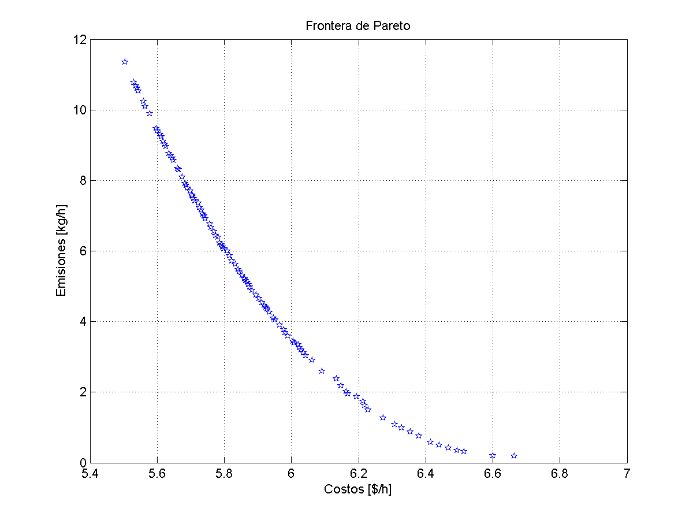
\includegraphics[width=0.3\textwidth,left]{logaritmica} 			
		  \end{figure}
		  
		\begin{figure}
			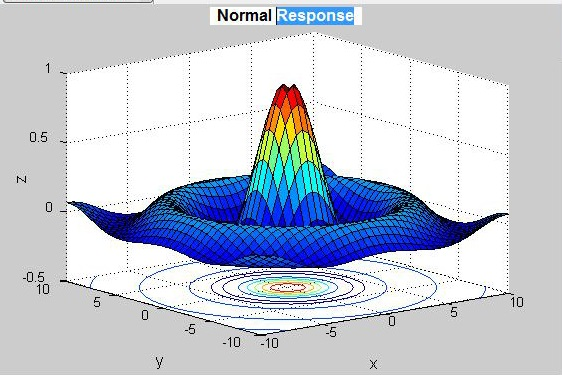
\includegraphics[width=0.3\textwidth]{curvas}
		\end{figure}
		\begin{figure}
			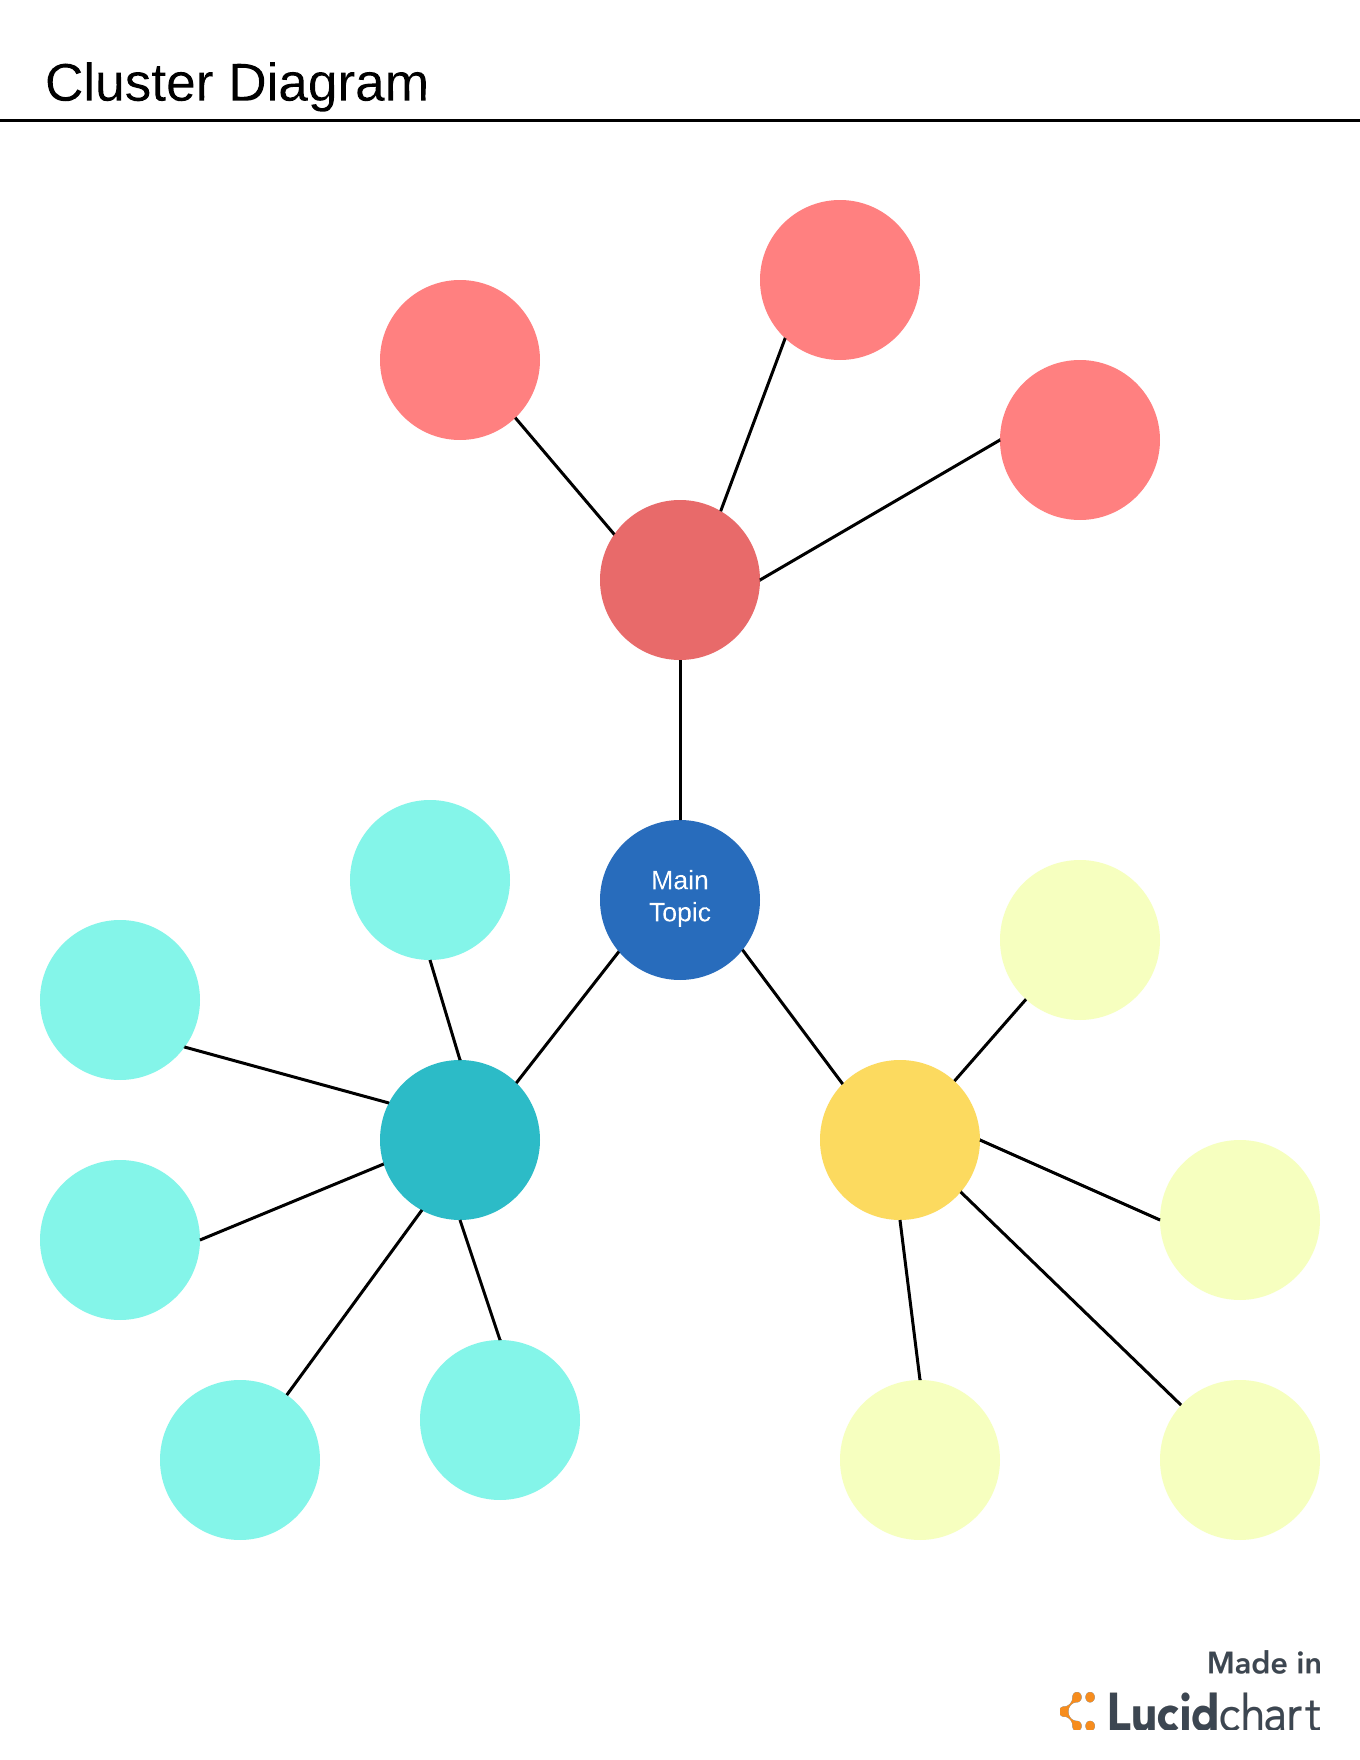
\includegraphics[width=0.3\textwidth, right]{red}
		\end{figure}
		
		  
	\end{frame}

\section{Resultados}
	\begin{frame}{Registros por año} 
		\begin{figure}
			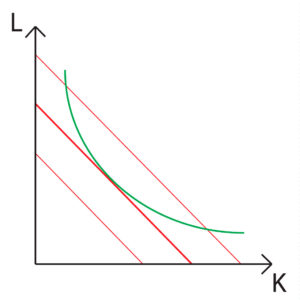
\includegraphics[width=0.5\textwidth]{grafico.jpg}
		\end{figure}
	\end{frame}


\section{Conclusiones y contribuciones}
	\begin{frame}{Conclusiones}
		\begin{itemize}
			\item Conclusión 1.
			\item Conclusión 2.
			\item Conclusión 3.
			\item Conclusión 4.
			\item Conclusión 5.
		\end{itemize}
	\end{frame}

	\begin{frame}{Contribuciones}
		\begin{itemize}
			\item Contribución $1$
			\item Contribución $2$
			\item Contribución $3$
			\item Contribución $4$
			\item Contribución $1$
		\end{itemize}
	\end{frame}

\section{Trabajo a futuro}
	\begin{frame}{Trabajo a futuro}
		\begin{itemize}
			\item Trabajo a futuro 1.
			\item Trabajo a futuro 2.
			\item Trabajo a futuro 3.
			\item Trabajo a futuro 4.
		\end{itemize}
	\end{frame}
\section{Agradecimientos}
	\begin{frame}
		\center{Gracias por su atención.} \\

		\begin{figure}
			
\includegraphics[width=0.4\textwidth]{adios.jpg}
		\end{figure}

		\url{su.correo@uanl.edu.mx}
		
	\end{frame}

\section{Bibliografía}
\begin{frame}[allowframebreaks]
	\bibliographystyle{apalike}
	\bibliography{Biblio}
\end{frame}


\end{document}
